% Options for packages loaded elsewhere
\PassOptionsToPackage{unicode}{hyperref}
\PassOptionsToPackage{hyphens}{url}
\PassOptionsToPackage{dvipsnames,svgnames,x11names}{xcolor}
%
\documentclass[
  letterpaper,
  DIV=11,
  numbers=noendperiod]{scrartcl}

\usepackage{amsmath,amssymb}
\usepackage{iftex}
\ifPDFTeX
  \usepackage[T1]{fontenc}
  \usepackage[utf8]{inputenc}
  \usepackage{textcomp} % provide euro and other symbols
\else % if luatex or xetex
  \usepackage{unicode-math}
  \defaultfontfeatures{Scale=MatchLowercase}
  \defaultfontfeatures[\rmfamily]{Ligatures=TeX,Scale=1}
\fi
\usepackage{lmodern}
\ifPDFTeX\else  
    % xetex/luatex font selection
\fi
% Use upquote if available, for straight quotes in verbatim environments
\IfFileExists{upquote.sty}{\usepackage{upquote}}{}
\IfFileExists{microtype.sty}{% use microtype if available
  \usepackage[]{microtype}
  \UseMicrotypeSet[protrusion]{basicmath} % disable protrusion for tt fonts
}{}
\makeatletter
\@ifundefined{KOMAClassName}{% if non-KOMA class
  \IfFileExists{parskip.sty}{%
    \usepackage{parskip}
  }{% else
    \setlength{\parindent}{0pt}
    \setlength{\parskip}{6pt plus 2pt minus 1pt}}
}{% if KOMA class
  \KOMAoptions{parskip=half}}
\makeatother
\usepackage{xcolor}
\setlength{\emergencystretch}{3em} % prevent overfull lines
\setcounter{secnumdepth}{-\maxdimen} % remove section numbering
% Make \paragraph and \subparagraph free-standing
\ifx\paragraph\undefined\else
  \let\oldparagraph\paragraph
  \renewcommand{\paragraph}[1]{\oldparagraph{#1}\mbox{}}
\fi
\ifx\subparagraph\undefined\else
  \let\oldsubparagraph\subparagraph
  \renewcommand{\subparagraph}[1]{\oldsubparagraph{#1}\mbox{}}
\fi

\usepackage{color}
\usepackage{fancyvrb}
\newcommand{\VerbBar}{|}
\newcommand{\VERB}{\Verb[commandchars=\\\{\}]}
\DefineVerbatimEnvironment{Highlighting}{Verbatim}{commandchars=\\\{\}}
% Add ',fontsize=\small' for more characters per line
\usepackage{framed}
\definecolor{shadecolor}{RGB}{241,243,245}
\newenvironment{Shaded}{\begin{snugshade}}{\end{snugshade}}
\newcommand{\AlertTok}[1]{\textcolor[rgb]{0.68,0.00,0.00}{#1}}
\newcommand{\AnnotationTok}[1]{\textcolor[rgb]{0.37,0.37,0.37}{#1}}
\newcommand{\AttributeTok}[1]{\textcolor[rgb]{0.40,0.45,0.13}{#1}}
\newcommand{\BaseNTok}[1]{\textcolor[rgb]{0.68,0.00,0.00}{#1}}
\newcommand{\BuiltInTok}[1]{\textcolor[rgb]{0.00,0.23,0.31}{#1}}
\newcommand{\CharTok}[1]{\textcolor[rgb]{0.13,0.47,0.30}{#1}}
\newcommand{\CommentTok}[1]{\textcolor[rgb]{0.37,0.37,0.37}{#1}}
\newcommand{\CommentVarTok}[1]{\textcolor[rgb]{0.37,0.37,0.37}{\textit{#1}}}
\newcommand{\ConstantTok}[1]{\textcolor[rgb]{0.56,0.35,0.01}{#1}}
\newcommand{\ControlFlowTok}[1]{\textcolor[rgb]{0.00,0.23,0.31}{#1}}
\newcommand{\DataTypeTok}[1]{\textcolor[rgb]{0.68,0.00,0.00}{#1}}
\newcommand{\DecValTok}[1]{\textcolor[rgb]{0.68,0.00,0.00}{#1}}
\newcommand{\DocumentationTok}[1]{\textcolor[rgb]{0.37,0.37,0.37}{\textit{#1}}}
\newcommand{\ErrorTok}[1]{\textcolor[rgb]{0.68,0.00,0.00}{#1}}
\newcommand{\ExtensionTok}[1]{\textcolor[rgb]{0.00,0.23,0.31}{#1}}
\newcommand{\FloatTok}[1]{\textcolor[rgb]{0.68,0.00,0.00}{#1}}
\newcommand{\FunctionTok}[1]{\textcolor[rgb]{0.28,0.35,0.67}{#1}}
\newcommand{\ImportTok}[1]{\textcolor[rgb]{0.00,0.46,0.62}{#1}}
\newcommand{\InformationTok}[1]{\textcolor[rgb]{0.37,0.37,0.37}{#1}}
\newcommand{\KeywordTok}[1]{\textcolor[rgb]{0.00,0.23,0.31}{#1}}
\newcommand{\NormalTok}[1]{\textcolor[rgb]{0.00,0.23,0.31}{#1}}
\newcommand{\OperatorTok}[1]{\textcolor[rgb]{0.37,0.37,0.37}{#1}}
\newcommand{\OtherTok}[1]{\textcolor[rgb]{0.00,0.23,0.31}{#1}}
\newcommand{\PreprocessorTok}[1]{\textcolor[rgb]{0.68,0.00,0.00}{#1}}
\newcommand{\RegionMarkerTok}[1]{\textcolor[rgb]{0.00,0.23,0.31}{#1}}
\newcommand{\SpecialCharTok}[1]{\textcolor[rgb]{0.37,0.37,0.37}{#1}}
\newcommand{\SpecialStringTok}[1]{\textcolor[rgb]{0.13,0.47,0.30}{#1}}
\newcommand{\StringTok}[1]{\textcolor[rgb]{0.13,0.47,0.30}{#1}}
\newcommand{\VariableTok}[1]{\textcolor[rgb]{0.07,0.07,0.07}{#1}}
\newcommand{\VerbatimStringTok}[1]{\textcolor[rgb]{0.13,0.47,0.30}{#1}}
\newcommand{\WarningTok}[1]{\textcolor[rgb]{0.37,0.37,0.37}{\textit{#1}}}

\providecommand{\tightlist}{%
  \setlength{\itemsep}{0pt}\setlength{\parskip}{0pt}}\usepackage{longtable,booktabs,array}
\usepackage{calc} % for calculating minipage widths
% Correct order of tables after \paragraph or \subparagraph
\usepackage{etoolbox}
\makeatletter
\patchcmd\longtable{\par}{\if@noskipsec\mbox{}\fi\par}{}{}
\makeatother
% Allow footnotes in longtable head/foot
\IfFileExists{footnotehyper.sty}{\usepackage{footnotehyper}}{\usepackage{footnote}}
\makesavenoteenv{longtable}
\usepackage{graphicx}
\makeatletter
\def\maxwidth{\ifdim\Gin@nat@width>\linewidth\linewidth\else\Gin@nat@width\fi}
\def\maxheight{\ifdim\Gin@nat@height>\textheight\textheight\else\Gin@nat@height\fi}
\makeatother
% Scale images if necessary, so that they will not overflow the page
% margins by default, and it is still possible to overwrite the defaults
% using explicit options in \includegraphics[width, height, ...]{}
\setkeys{Gin}{width=\maxwidth,height=\maxheight,keepaspectratio}
% Set default figure placement to htbp
\makeatletter
\def\fps@figure{htbp}
\makeatother

\KOMAoption{captions}{tableheading}
\makeatletter
\makeatother
\makeatletter
\makeatother
\makeatletter
\@ifpackageloaded{caption}{}{\usepackage{caption}}
\AtBeginDocument{%
\ifdefined\contentsname
  \renewcommand*\contentsname{Table of contents}
\else
  \newcommand\contentsname{Table of contents}
\fi
\ifdefined\listfigurename
  \renewcommand*\listfigurename{List of Figures}
\else
  \newcommand\listfigurename{List of Figures}
\fi
\ifdefined\listtablename
  \renewcommand*\listtablename{List of Tables}
\else
  \newcommand\listtablename{List of Tables}
\fi
\ifdefined\figurename
  \renewcommand*\figurename{Figure}
\else
  \newcommand\figurename{Figure}
\fi
\ifdefined\tablename
  \renewcommand*\tablename{Table}
\else
  \newcommand\tablename{Table}
\fi
}
\@ifpackageloaded{float}{}{\usepackage{float}}
\floatstyle{ruled}
\@ifundefined{c@chapter}{\newfloat{codelisting}{h}{lop}}{\newfloat{codelisting}{h}{lop}[chapter]}
\floatname{codelisting}{Listing}
\newcommand*\listoflistings{\listof{codelisting}{List of Listings}}
\makeatother
\makeatletter
\@ifpackageloaded{caption}{}{\usepackage{caption}}
\@ifpackageloaded{subcaption}{}{\usepackage{subcaption}}
\makeatother
\makeatletter
\@ifpackageloaded{tcolorbox}{}{\usepackage[skins,breakable]{tcolorbox}}
\makeatother
\makeatletter
\@ifundefined{shadecolor}{\definecolor{shadecolor}{rgb}{.97, .97, .97}}
\makeatother
\makeatletter
\makeatother
\makeatletter
\makeatother
\ifLuaTeX
  \usepackage{selnolig}  % disable illegal ligatures
\fi
\IfFileExists{bookmark.sty}{\usepackage{bookmark}}{\usepackage{hyperref}}
\IfFileExists{xurl.sty}{\usepackage{xurl}}{} % add URL line breaks if available
\urlstyle{same} % disable monospaced font for URLs
\hypersetup{
  pdftitle={Assignment 3},
  pdfauthor={Group 2},
  colorlinks=true,
  linkcolor={blue},
  filecolor={Maroon},
  citecolor={Blue},
  urlcolor={Blue},
  pdfcreator={LaTeX via pandoc}}

\title{Assignment 3}
\author{Group 2}
\date{2024-03-18}

\begin{document}
\maketitle
\ifdefined\Shaded\renewenvironment{Shaded}{\begin{tcolorbox}[borderline west={3pt}{0pt}{shadecolor}, frame hidden, boxrule=0pt, breakable, interior hidden, sharp corners, enhanced]}{\end{tcolorbox}}\fi

\begin{Shaded}
\begin{Highlighting}[]
\FunctionTok{library}\NormalTok{(tidycensus)}
\FunctionTok{library}\NormalTok{(tidyverse)}
\FunctionTok{library}\NormalTok{(tidymodels) }\CommentTok{\# collection of packages for machine learning }
\FunctionTok{library}\NormalTok{(kknn) }\CommentTok{\# package for k{-}nearest neighbors models}
\FunctionTok{library}\NormalTok{(sf)}
\end{Highlighting}
\end{Shaded}

\begin{Shaded}
\begin{Highlighting}[]
\NormalTok{vars }\OtherTok{\textless{}{-}} \FunctionTok{c}\NormalTok{(}
  \StringTok{"B06011\_001E"}\NormalTok{, }\CommentTok{\# mean income}
  \StringTok{"B19122\_001E"}\NormalTok{, }\CommentTok{\# household earner}
  \StringTok{"DP03\_0025E"}\NormalTok{, }\CommentTok{\# Median Gross Rent (Dollars)}
  \StringTok{"B25064\_001E"}\NormalTok{, }\CommentTok{\# Mean travel time to work (minutes)}
  \StringTok{"B19058\_001E"}\NormalTok{,}\CommentTok{\# Public Assistance Income or Food Stamps/SNAP in the Past 12 Months for Households }
  \StringTok{"DP02\_0068E"}\NormalTok{,}\CommentTok{\# Total population over 25 years with bachelor\textquotesingle{}s degree or higher}
  \StringTok{"DP02\_0059E"}\NormalTok{, }\CommentTok{\# Total population over 25 years}
  \StringTok{"DP03\_0048PE"}\NormalTok{, }\CommentTok{\# Civilian employed population 16 years and over}
  \StringTok{"B17001\_001E"}\NormalTok{, }\CommentTok{\# total\_pop}
  \StringTok{"B17001\_002E"} \CommentTok{\# below\_poverty}
\NormalTok{  )}

\NormalTok{ACS }\OtherTok{\textless{}{-}} \FunctionTok{get\_acs}\NormalTok{(}\AttributeTok{geography =} \StringTok{"county"}\NormalTok{, }
                    \AttributeTok{variables =}\NormalTok{ vars, }
                    \AttributeTok{year =} \DecValTok{2022}\NormalTok{,}
                    \AttributeTok{survey =} \StringTok{"acs1"}\NormalTok{, }
                    \AttributeTok{output =} \StringTok{"wide"}\NormalTok{)}

\NormalTok{LAT\_train }\OtherTok{\textless{}{-}}\NormalTok{ readxl}\SpecialCharTok{::}\FunctionTok{read\_xlsx}\NormalTok{(}\StringTok{"Data Raw/Labor action tracker data 12.4.23.xlsx"}\NormalTok{)}
\NormalTok{LAT\_test }\OtherTok{\textless{}{-}}\NormalTok{ readxl}\SpecialCharTok{::}\FunctionTok{read\_xlsx}\NormalTok{(}\StringTok{"Data Raw/Labor action tracker data 2.26.24.xlsx"}\NormalTok{)}
\end{Highlighting}
\end{Shaded}

\begin{Shaded}
\begin{Highlighting}[]
\NormalTok{county }\OtherTok{\textless{}{-}}\NormalTok{ tigris}\SpecialCharTok{::}\FunctionTok{counties}\NormalTok{(}\AttributeTok{cb =} \ConstantTok{TRUE}\NormalTok{)}
\CommentTok{\#{-}{-}{-}{-}{-}{-}{-}{-}{-}{-}}
\CommentTok{\# LAT Train Data}
\CommentTok{\#{-}{-}{-}{-}{-}{-}{-}{-}{-}{-}}
\NormalTok{LAT\_train }\OtherTok{\textless{}{-}}\NormalTok{ LAT\_train }\SpecialCharTok{\%\textgreater{}\%}
  \FunctionTok{mutate}\NormalTok{(}
    \AttributeTok{coordinate =} \FunctionTok{ifelse}\NormalTok{(}
      \StringTok{\textasciigrave{}}\AttributeTok{Number of Locations}\StringTok{\textasciigrave{}} \SpecialCharTok{\textgreater{}} \DecValTok{1}\NormalTok{,}
      \FunctionTok{strsplit}\NormalTok{(}\FunctionTok{as.character}\NormalTok{(}\StringTok{\textasciigrave{}}\AttributeTok{Latitude, Longitude}\StringTok{\textasciigrave{}}\NormalTok{), }\StringTok{";}\SpecialCharTok{\textbackslash{}\textbackslash{}}\StringTok{s*"}\NormalTok{),}
      \StringTok{\textasciigrave{}}\AttributeTok{Latitude, Longitude}\StringTok{\textasciigrave{}}
\NormalTok{    ))}\SpecialCharTok{\%\textgreater{}\%}  
  \FunctionTok{unnest}\NormalTok{(coordinate)}
\NormalTok{LAT\_train }\OtherTok{\textless{}{-}} \FunctionTok{separate}\NormalTok{(LAT\_train, coordinate, }\AttributeTok{into =} \FunctionTok{c}\NormalTok{(}\StringTok{"lat"}\NormalTok{, }\StringTok{"lon"}\NormalTok{), }
                 \AttributeTok{sep =} \StringTok{",}\SpecialCharTok{\textbackslash{}\textbackslash{}}\StringTok{s*"}\NormalTok{, }\AttributeTok{remove =} \ConstantTok{FALSE}\NormalTok{)}
\CommentTok{\# check is there any NAs }
\NormalTok{LAT\_train }\OtherTok{\textless{}{-}}\NormalTok{ LAT\_train }\SpecialCharTok{\%\textgreater{}\%}
  \FunctionTok{mutate}\NormalTok{(}
    \AttributeTok{lat =} \FunctionTok{as.numeric}\NormalTok{(lat),}
    \AttributeTok{lon =} \FunctionTok{as.numeric}\NormalTok{(lon))}
\NormalTok{na\_summary }\OtherTok{\textless{}{-}}\NormalTok{ LAT\_train }\SpecialCharTok{\%\textgreater{}\%}
  \FunctionTok{summarise\_all}\NormalTok{(}\SpecialCharTok{\textasciitilde{}} \FunctionTok{sum}\NormalTok{(}\FunctionTok{is.na}\NormalTok{(.)))}
\CommentTok{\# yes, there is one in lon column. }
\NormalTok{LAT\_train}\SpecialCharTok{$}\NormalTok{lon[}\DecValTok{2830}\NormalTok{] }\OtherTok{=} \SpecialCharTok{{-}}\FloatTok{85.73642799999999}
\CommentTok{\# transform LAT data into geometric data frame}
\NormalTok{LAT\_train }\OtherTok{\textless{}{-}} \FunctionTok{st\_as\_sf}\NormalTok{(LAT\_train, }\AttributeTok{coords =} \FunctionTok{c}\NormalTok{(}\StringTok{"lon"}\NormalTok{, }\StringTok{"lat"}\NormalTok{))}
\CommentTok{\# matching same projection}
\FunctionTok{st\_crs}\NormalTok{(LAT\_train) }\OtherTok{\textless{}{-}} \FunctionTok{st\_crs}\NormalTok{(county)}
\CommentTok{\# joining 2 geometric data frames}
\NormalTok{LAT\_train }\OtherTok{\textless{}{-}} \FunctionTok{st\_join}\NormalTok{(LAT\_train, county)}
\CommentTok{\# housekeeping and make LAT data looks clean and organized}
\NormalTok{vars }\OtherTok{\textless{}{-}} \FunctionTok{names}\NormalTok{(LAT\_train)}
\NormalTok{LAT\_train }\OtherTok{\textless{}{-}}\NormalTok{ LAT\_train }\SpecialCharTok{\%\textgreater{}\%}
  \FunctionTok{select}\NormalTok{(}\FunctionTok{c}\NormalTok{(}\FunctionTok{all\_of}\NormalTok{(vars), NAMELSAD, GEOID)) }\SpecialCharTok{\%\textgreater{}\%}
  \FunctionTok{rename}\NormalTok{(}\AttributeTok{County =}\NormalTok{ NAMELSAD) }\SpecialCharTok{\%\textgreater{}\%}
  \FunctionTok{select}\NormalTok{(}\DecValTok{1}\SpecialCharTok{:}\DecValTok{10}\NormalTok{, }\DecValTok{23}\NormalTok{, }\DecValTok{11}\SpecialCharTok{:}\DecValTok{22}\NormalTok{, }\DecValTok{24}\NormalTok{, }\DecValTok{29}\NormalTok{, }\DecValTok{31}\NormalTok{)}

\CommentTok{\#{-}{-}{-}{-}{-}{-}{-}{-}{-}{-}}
\CommentTok{\# LAT Test Data}
\CommentTok{\#{-}{-}{-}{-}{-}{-}{-}{-}{-}{-}}
\NormalTok{LAT\_test }\OtherTok{\textless{}{-}}\NormalTok{ LAT\_test }\SpecialCharTok{\%\textgreater{}\%}
  \FunctionTok{mutate}\NormalTok{(}
    \AttributeTok{coordinate =} \FunctionTok{ifelse}\NormalTok{(}
      \StringTok{\textasciigrave{}}\AttributeTok{Number of Locations}\StringTok{\textasciigrave{}} \SpecialCharTok{\textgreater{}} \DecValTok{1}\NormalTok{,}
      \FunctionTok{strsplit}\NormalTok{(}\FunctionTok{as.character}\NormalTok{(}\StringTok{\textasciigrave{}}\AttributeTok{Latitude, Longitude}\StringTok{\textasciigrave{}}\NormalTok{), }\StringTok{";}\SpecialCharTok{\textbackslash{}\textbackslash{}}\StringTok{s*"}\NormalTok{),}
      \StringTok{\textasciigrave{}}\AttributeTok{Latitude, Longitude}\StringTok{\textasciigrave{}}
\NormalTok{    ))}\SpecialCharTok{\%\textgreater{}\%}  
  \FunctionTok{unnest}\NormalTok{(coordinate)}
\NormalTok{LAT\_test }\OtherTok{\textless{}{-}} \FunctionTok{separate}\NormalTok{(LAT\_test, coordinate, }\AttributeTok{into =} \FunctionTok{c}\NormalTok{(}\StringTok{"lat"}\NormalTok{, }\StringTok{"lon"}\NormalTok{), }
                 \AttributeTok{sep =} \StringTok{",}\SpecialCharTok{\textbackslash{}\textbackslash{}}\StringTok{s*"}\NormalTok{, }\AttributeTok{remove =} \ConstantTok{FALSE}\NormalTok{)}
\CommentTok{\# check is there any NAs }
\NormalTok{LAT\_test }\OtherTok{\textless{}{-}}\NormalTok{ LAT\_test }\SpecialCharTok{\%\textgreater{}\%}
  \FunctionTok{mutate}\NormalTok{(}
    \AttributeTok{lat =} \FunctionTok{as.numeric}\NormalTok{(lat),}
    \AttributeTok{lon =} \FunctionTok{as.numeric}\NormalTok{(lon))}
\NormalTok{na\_summary }\OtherTok{\textless{}{-}}\NormalTok{ LAT\_test }\SpecialCharTok{\%\textgreater{}\%}
  \FunctionTok{summarise\_all}\NormalTok{(}\SpecialCharTok{\textasciitilde{}} \FunctionTok{sum}\NormalTok{(}\FunctionTok{is.na}\NormalTok{(.))) }\CommentTok{\# There is no NAs}

\NormalTok{LAT\_test }\OtherTok{\textless{}{-}} \FunctionTok{st\_as\_sf}\NormalTok{(LAT\_test, }\AttributeTok{coords =} \FunctionTok{c}\NormalTok{(}\StringTok{"lon"}\NormalTok{, }\StringTok{"lat"}\NormalTok{))}
\CommentTok{\# matching same projection}
\FunctionTok{st\_crs}\NormalTok{(LAT\_test) }\OtherTok{\textless{}{-}} \FunctionTok{st\_crs}\NormalTok{(county)}
\CommentTok{\# joining 2 geometric data frames}
\NormalTok{LAT\_test }\OtherTok{\textless{}{-}} \FunctionTok{st\_join}\NormalTok{(LAT\_test, county)}
\CommentTok{\# housekeeping and make LAT data looks clean and organized}
\NormalTok{vars }\OtherTok{\textless{}{-}} \FunctionTok{names}\NormalTok{(LAT\_test)}
\NormalTok{LAT\_test }\OtherTok{\textless{}{-}}\NormalTok{ LAT\_test }\SpecialCharTok{\%\textgreater{}\%}
  \FunctionTok{select}\NormalTok{(}\FunctionTok{c}\NormalTok{(}\FunctionTok{all\_of}\NormalTok{(vars), NAMELSAD, GEOID)) }\SpecialCharTok{\%\textgreater{}\%}
  \FunctionTok{rename}\NormalTok{(}\AttributeTok{County =}\NormalTok{ NAMELSAD) }\SpecialCharTok{\%\textgreater{}\%}
  \FunctionTok{select}\NormalTok{(}\DecValTok{1}\SpecialCharTok{:}\DecValTok{10}\NormalTok{, }\DecValTok{23}\NormalTok{, }\DecValTok{11}\SpecialCharTok{:}\DecValTok{22}\NormalTok{, }\DecValTok{24}\NormalTok{, }\DecValTok{29}\NormalTok{, }\DecValTok{31}\NormalTok{)}
\end{Highlighting}
\end{Shaded}

\begin{Shaded}
\begin{Highlighting}[]
\NormalTok{ACS }\OtherTok{\textless{}{-}}\NormalTok{ ACS }\SpecialCharTok{\%\textgreater{}\%}  
  \FunctionTok{select}\NormalTok{(GEOID, }\FunctionTok{ends\_with}\NormalTok{(}\StringTok{"E"}\NormalTok{)) }\SpecialCharTok{\%\textgreater{}\%}
  \FunctionTok{separate}\NormalTok{(}\AttributeTok{col =} \StringTok{"NAME"}\NormalTok{, }\AttributeTok{into =} \FunctionTok{c}\NormalTok{(}\StringTok{"County"}\NormalTok{, }\StringTok{"State"}\NormalTok{), }\AttributeTok{sep =} \StringTok{","}\NormalTok{) }\SpecialCharTok{\%\textgreater{}\%}
  \FunctionTok{rename}\NormalTok{(}
    \StringTok{"median\_inc"} \OtherTok{=} \StringTok{"B06011\_001E"}\NormalTok{,}
    \StringTok{"earners"} \OtherTok{=} \StringTok{"B19122\_001E"}\NormalTok{,}
    \StringTok{"travel\_work"}\OtherTok{=}\StringTok{"DP03\_0025E"}\NormalTok{,}
    \StringTok{"total\_pop"} \OtherTok{=} \StringTok{"B17001\_001E"}\NormalTok{,}
    \StringTok{"below\_poverty"} \OtherTok{=} \StringTok{"B17001\_002E"}\NormalTok{,}
    \StringTok{"rent"} \OtherTok{=} \StringTok{"B25064\_001E"}\NormalTok{,}
    \StringTok{"assi\_income"}\OtherTok{=} \StringTok{"B19058\_001E"}\NormalTok{,}
    \StringTok{"ba\_pop"}\OtherTok{=} \StringTok{"DP02\_0068E"}\NormalTok{,}
    \StringTok{"total\_pop25"}\OtherTok{=}\StringTok{"DP02\_0059E"}\NormalTok{,}
    \StringTok{"employed"}\OtherTok{=}\StringTok{"DP03\_0048PE"} \CommentTok{\# Civilian employed population 16 years and over}
\NormalTok{) }\SpecialCharTok{\%\textgreater{}\%}
  \FunctionTok{mutate}\NormalTok{(}
    \AttributeTok{poverty\_rate =}\NormalTok{ below\_poverty}\SpecialCharTok{/}\NormalTok{total\_pop,}
    \AttributeTok{ba\_rate =}\NormalTok{ ba\_pop}\SpecialCharTok{/}\NormalTok{total\_pop}
\NormalTok{  )}
\end{Highlighting}
\end{Shaded}

\begin{Shaded}
\begin{Highlighting}[]
\CommentTok{\#Here is the final data set with all acs variables and the LAT data}
\CommentTok{\#Since around 90\% of the duration was NAs, so I did not unify the time into a new column.}

\NormalTok{data\_train }\OtherTok{\textless{}{-}} \FunctionTok{left\_join}\NormalTok{(LAT\_train, ACS, }\AttributeTok{by=}\StringTok{"GEOID"}\NormalTok{)}
\NormalTok{data\_train }\OtherTok{\textless{}{-}} \FunctionTok{as.data.frame}\NormalTok{(data\_train)}
\CommentTok{\# clean out redundant variables}
\NormalTok{data\_train }\OtherTok{\textless{}{-}}\NormalTok{ data\_train  }\SpecialCharTok{\%\textgreater{}\%}
  \FunctionTok{select}\NormalTok{(}\SpecialCharTok{{-}}\FunctionTok{ends\_with}\NormalTok{(}\StringTok{".x"}\NormalTok{)) }\SpecialCharTok{\%\textgreater{}\%}
  \FunctionTok{select}\NormalTok{(}\SpecialCharTok{{-}}\FunctionTok{ends\_with}\NormalTok{(}\StringTok{".y"}\NormalTok{))}

\NormalTok{data\_test }\OtherTok{\textless{}{-}} \FunctionTok{left\_join}\NormalTok{(LAT\_test, ACS, }\AttributeTok{by=}\StringTok{"GEOID"}\NormalTok{)}
\NormalTok{data\_test }\OtherTok{\textless{}{-}} \FunctionTok{as.data.frame}\NormalTok{(data\_test)}
\CommentTok{\# clean out redundant variables}
\NormalTok{data\_test }\OtherTok{\textless{}{-}}\NormalTok{ data\_test  }\SpecialCharTok{\%\textgreater{}\%}
  \FunctionTok{select}\NormalTok{(}\SpecialCharTok{{-}}\FunctionTok{ends\_with}\NormalTok{(}\StringTok{".x"}\NormalTok{)) }\SpecialCharTok{\%\textgreater{}\%}
  \FunctionTok{select}\NormalTok{(}\SpecialCharTok{{-}}\FunctionTok{ends\_with}\NormalTok{(}\StringTok{".y"}\NormalTok{))}

\CommentTok{\# A new column I combine the other two labor actions into non{-}strike }
\NormalTok{data\_train }\OtherTok{\textless{}{-}}\NormalTok{ data\_train }\SpecialCharTok{\%\textgreater{}\%} 
  \FunctionTok{mutate}\NormalTok{(}\AttributeTok{Strike\_or\_not =} \FunctionTok{ifelse}\NormalTok{(}\StringTok{\textasciigrave{}}\AttributeTok{Strike or Protest}\StringTok{\textasciigrave{}}\SpecialCharTok{==} \StringTok{"Strike"}\NormalTok{,}\DecValTok{1}\NormalTok{,}\DecValTok{0}\NormalTok{))}
\NormalTok{data\_test }\OtherTok{\textless{}{-}}\NormalTok{ data\_test }\SpecialCharTok{\%\textgreater{}\%} 
  \FunctionTok{mutate}\NormalTok{(}\AttributeTok{Strike\_or\_not =} \FunctionTok{ifelse}\NormalTok{(}\StringTok{\textasciigrave{}}\AttributeTok{Strike or Protest}\StringTok{\textasciigrave{}}\SpecialCharTok{==} \StringTok{"Strike"}\NormalTok{,}\DecValTok{1}\NormalTok{,}\DecValTok{0}\NormalTok{))}

\FunctionTok{write\_csv}\NormalTok{(data\_train, }\StringTok{"Data Clean/data\_train.csv"}\NormalTok{)}
\FunctionTok{write\_csv}\NormalTok{(data\_test, }\StringTok{"Data Clean/data\_test.csv"}\NormalTok{)}
\end{Highlighting}
\end{Shaded}

\begin{Shaded}
\begin{Highlighting}[]
\FunctionTok{set.seed}\NormalTok{(}\DecValTok{100}\NormalTok{)}

\NormalTok{data\_train }\OtherTok{\textless{}{-}}\NormalTok{ data\_train }\SpecialCharTok{\%\textgreater{}\%} \FunctionTok{mutate}\NormalTok{(}\AttributeTok{Strike\_or\_not\_f =} \FunctionTok{as.factor}\NormalTok{(Strike\_or\_not))}
\NormalTok{data\_test }\OtherTok{\textless{}{-}}\NormalTok{ data\_test }\SpecialCharTok{\%\textgreater{}\%} \FunctionTok{mutate}\NormalTok{(}\AttributeTok{Strike\_or\_not\_f =} \FunctionTok{as.factor}\NormalTok{(Strike\_or\_not))}

\CommentTok{\# Defining the "recipe" to preprocess the data}

\NormalTok{recipe }\OtherTok{\textless{}{-}} \FunctionTok{recipe}\NormalTok{(Strike\_or\_not\_f }\SpecialCharTok{\textasciitilde{}}\NormalTok{ median\_inc }\SpecialCharTok{+}\NormalTok{ earners }\SpecialCharTok{+}\NormalTok{ travel\_work }\SpecialCharTok{+}\NormalTok{ rent }\SpecialCharTok{+}
\NormalTok{          assi\_income }\SpecialCharTok{+}\NormalTok{ employed}\SpecialCharTok{+}\NormalTok{poverty\_rate}\SpecialCharTok{+}\NormalTok{ba\_rate, }
                 \AttributeTok{data =}\NormalTok{ data\_train) }\SpecialCharTok{|\textgreater{}}
  \FunctionTok{step\_scale}\NormalTok{(}\FunctionTok{all\_predictors}\NormalTok{()) }\SpecialCharTok{|\textgreater{}} \CommentTok{\# Normalizing standard deviation to one}
  \FunctionTok{step\_impute\_mean}\NormalTok{(}\FunctionTok{all\_predictors}\NormalTok{()) }\CommentTok{\# Normalizing mean to one}


\CommentTok{\# KNN Model 1}

\NormalTok{model1 }\OtherTok{\textless{}{-}} \FunctionTok{nearest\_neighbor}\NormalTok{(}
  \AttributeTok{mode =} \StringTok{"classification"}\NormalTok{, }\CommentTok{\# Our Y is categorical, so we use classification}
  \AttributeTok{engine =} \StringTok{"kknn"}\NormalTok{, }\CommentTok{\# Engine for KNN used by tidymodels}
  \AttributeTok{neighbors =} \DecValTok{59}\NormalTok{) }\CommentTok{\# sqrt n}


\CommentTok{\# Setting up the workflow}

\NormalTok{workflow1 }\OtherTok{\textless{}{-}} \FunctionTok{workflow}\NormalTok{() }\SpecialCharTok{|\textgreater{}}
  \FunctionTok{add\_recipe}\NormalTok{(recipe) }\SpecialCharTok{|\textgreater{}}
  \FunctionTok{add\_model}\NormalTok{(model1)}


\CommentTok{\# Fitting model to training data}

\NormalTok{fit1 }\OtherTok{\textless{}{-}}\NormalTok{ workflow1 }\SpecialCharTok{|\textgreater{}}
  \FunctionTok{fit}\NormalTok{(}\AttributeTok{data =}\NormalTok{ data\_train)}


\CommentTok{\# Making predictions on the testing data}

\NormalTok{preds\_test }\OtherTok{\textless{}{-}} \FunctionTok{predict}\NormalTok{(fit1, }
                      \AttributeTok{new\_data =}\NormalTok{ data\_test, }
                      \AttributeTok{type =} \StringTok{"class"}\NormalTok{) }\CommentTok{\# Classification}

\CommentTok{\# Binding the actual and predicted Y\textquotesingle{}s together in data frames}

\NormalTok{df\_eval\_test }\OtherTok{\textless{}{-}} \FunctionTok{cbind}\NormalTok{(}\StringTok{"pop"} \OtherTok{=}\NormalTok{ data\_test}\SpecialCharTok{$}\NormalTok{Strike\_or\_not\_f, preds\_test)}


\CommentTok{\# Evaluating the models with confusion matrices}

\NormalTok{cm\_test1 }\OtherTok{\textless{}{-}} \FunctionTok{conf\_mat}\NormalTok{(}\AttributeTok{data =}\NormalTok{ df\_eval\_test,}
                    \AttributeTok{truth =}\NormalTok{ pop, }
                    \AttributeTok{estimate =}\NormalTok{ .pred\_class)}

\CommentTok{\# Printing confusion matrices}

\FunctionTok{print}\NormalTok{(}\StringTok{"Confusion matrix for testing data:"}\NormalTok{)}
\end{Highlighting}
\end{Shaded}

\begin{verbatim}
[1] "Confusion matrix for testing data:"
\end{verbatim}

\begin{Shaded}
\begin{Highlighting}[]
\NormalTok{cm\_test1}
\end{Highlighting}
\end{Shaded}

\begin{verbatim}
          Truth
Prediction   0   1
         0 108  84
         1  44  76
\end{verbatim}

\begin{Shaded}
\begin{Highlighting}[]
\CommentTok{\#{-}{-}{-}{-}{-}{-}{-}{-}{-}{-}{-}{-}{-}{-}{-}{-}{-}{-}{-}{-}{-}{-}{-}{-}{-}{-}{-}{-}{-}{-}{-}{-}{-}{-}{-}{-}{-}{-}{-}{-}{-}{-}{-}{-}{-}{-}{-}{-}{-}{-}{-}{-}{-}{-}{-}{-}{-}{-}{-}{-}{-}{-}{-}{-}{-}{-}{-}{-}{-}{-}{-}{-}{-}{-}{-}{-}{-}{-}{-}}

\CommentTok{\# KNN Model 2}

\NormalTok{model2 }\OtherTok{\textless{}{-}} \FunctionTok{nearest\_neighbor}\NormalTok{(}
  \AttributeTok{mode =} \StringTok{"classification"}\NormalTok{, }\CommentTok{\# Our Y is categorical, so we use classification}
  \AttributeTok{engine =} \StringTok{"kknn"}\NormalTok{, }\CommentTok{\# Engine for KNN used by tidymodels}
  \AttributeTok{neighbors =} \DecValTok{29}\NormalTok{) }\CommentTok{\# sqrt n/2}


\CommentTok{\# Setting up the workflow}

\NormalTok{workflow2 }\OtherTok{\textless{}{-}} \FunctionTok{workflow}\NormalTok{() }\SpecialCharTok{|\textgreater{}}
  \FunctionTok{add\_recipe}\NormalTok{(recipe) }\SpecialCharTok{|\textgreater{}}
  \FunctionTok{add\_model}\NormalTok{(model2)}


\CommentTok{\# Fitting model to training data}

\NormalTok{fit2 }\OtherTok{\textless{}{-}}\NormalTok{ workflow2 }\SpecialCharTok{|\textgreater{}}
  \FunctionTok{fit}\NormalTok{(}\AttributeTok{data =}\NormalTok{ data\_train)}


\CommentTok{\# Making predictions on the testing data}

\NormalTok{preds\_test }\OtherTok{\textless{}{-}} \FunctionTok{predict}\NormalTok{(fit2, }
                      \AttributeTok{new\_data =}\NormalTok{ data\_test, }
                      \AttributeTok{type =} \StringTok{"class"}\NormalTok{) }\CommentTok{\# Classification}

\CommentTok{\# Binding the actual and predicted Y\textquotesingle{}s together in data frames}

\NormalTok{df\_eval\_test }\OtherTok{\textless{}{-}} \FunctionTok{cbind}\NormalTok{(}\StringTok{"pop"} \OtherTok{=}\NormalTok{ data\_test}\SpecialCharTok{$}\NormalTok{Strike\_or\_not\_f, preds\_test)}


\CommentTok{\# Evaluating the models with confusion matrices}

\NormalTok{cm\_test2 }\OtherTok{\textless{}{-}} \FunctionTok{conf\_mat}\NormalTok{(}\AttributeTok{data =}\NormalTok{ df\_eval\_test,}
                    \AttributeTok{truth =}\NormalTok{ pop, }
                    \AttributeTok{estimate =}\NormalTok{ .pred\_class)}

\CommentTok{\# Printing confusion matrices}

\FunctionTok{print}\NormalTok{(}\StringTok{"Confusion matrix for testing data:"}\NormalTok{)}
\end{Highlighting}
\end{Shaded}

\begin{verbatim}
[1] "Confusion matrix for testing data:"
\end{verbatim}

\begin{Shaded}
\begin{Highlighting}[]
\NormalTok{cm\_test2}
\end{Highlighting}
\end{Shaded}

\begin{verbatim}
          Truth
Prediction   0   1
         0 108  89
         1  44  71
\end{verbatim}

\begin{Shaded}
\begin{Highlighting}[]
\CommentTok{\#{-}{-}{-}{-}{-}{-}{-}{-}{-}{-}{-}{-}{-}{-}{-}{-}{-}{-}{-}{-}{-}{-}{-}{-}{-}{-}{-}{-}{-}{-}{-}{-}{-}{-}{-}{-}{-}{-}{-}{-}{-}{-}{-}{-}{-}{-}{-}{-}{-}{-}{-}{-}{-}{-}{-}{-}{-}{-}{-}{-}{-}{-}{-}{-}{-}{-}{-}{-}{-}{-}{-}{-}{-}{-}{-}{-}{-}{-}{-}}

\CommentTok{\# KNN Model 3}

\NormalTok{model3 }\OtherTok{\textless{}{-}} \FunctionTok{nearest\_neighbor}\NormalTok{(}
  \AttributeTok{mode =} \StringTok{"classification"}\NormalTok{, }\CommentTok{\# Our Y is categorical, so we use classification}
  \AttributeTok{engine =} \StringTok{"kknn"}\NormalTok{, }\CommentTok{\# Engine for KNN used by tidymodels}
  \AttributeTok{neighbors =} \DecValTok{119}\NormalTok{) }\CommentTok{\# sqrt n*2}


\CommentTok{\# Setting up the workflow}

\NormalTok{workflow3 }\OtherTok{\textless{}{-}} \FunctionTok{workflow}\NormalTok{() }\SpecialCharTok{|\textgreater{}}
  \FunctionTok{add\_recipe}\NormalTok{(recipe) }\SpecialCharTok{|\textgreater{}}
  \FunctionTok{add\_model}\NormalTok{(model3)}


\CommentTok{\# Fitting model to training data}

\NormalTok{fit3 }\OtherTok{\textless{}{-}}\NormalTok{ workflow3 }\SpecialCharTok{|\textgreater{}}
  \FunctionTok{fit}\NormalTok{(}\AttributeTok{data =}\NormalTok{ data\_train)}


\CommentTok{\# Making predictions on the testing data}

\NormalTok{preds\_test }\OtherTok{\textless{}{-}} \FunctionTok{predict}\NormalTok{(fit3, }
                      \AttributeTok{new\_data =}\NormalTok{ data\_test, }
                      \AttributeTok{type =} \StringTok{"class"}\NormalTok{) }\CommentTok{\# Classification}

\CommentTok{\# Binding the actual and predicted Y\textquotesingle{}s together in data frames}

\NormalTok{df\_eval\_test }\OtherTok{\textless{}{-}} \FunctionTok{cbind}\NormalTok{(}\StringTok{"pop"} \OtherTok{=}\NormalTok{ data\_test}\SpecialCharTok{$}\NormalTok{Strike\_or\_not\_f, preds\_test)}


\CommentTok{\# Evaluating the models with confusion matrices}

\NormalTok{cm\_test3 }\OtherTok{\textless{}{-}} \FunctionTok{conf\_mat}\NormalTok{(}\AttributeTok{data =}\NormalTok{ df\_eval\_test,}
                    \AttributeTok{truth =}\NormalTok{ pop, }
                    \AttributeTok{estimate =}\NormalTok{ .pred\_class)}

\CommentTok{\# Printing confusion matrices}

\FunctionTok{print}\NormalTok{(}\StringTok{"Confusion matrix for testing data:"}\NormalTok{)}
\end{Highlighting}
\end{Shaded}

\begin{verbatim}
[1] "Confusion matrix for testing data:"
\end{verbatim}

\begin{Shaded}
\begin{Highlighting}[]
\NormalTok{cm\_test3}
\end{Highlighting}
\end{Shaded}

\begin{verbatim}
          Truth
Prediction   0   1
         0 104  78
         1  48  82
\end{verbatim}

\begin{Shaded}
\begin{Highlighting}[]
\CommentTok{\#{-}{-}{-}{-}{-}{-}{-}{-}{-}{-}{-}{-}{-}{-}{-}{-}{-}{-}{-}{-}{-}{-}{-}{-}{-}{-}{-}{-}{-}{-}{-}{-}{-}{-}{-}{-}{-}{-}{-}{-}{-}{-}{-}{-}{-}{-}{-}{-}{-}{-}{-}{-}{-}{-}{-}{-}{-}{-}{-}{-}{-}{-}{-}{-}{-}{-}{-}{-}{-}{-}{-}{-}{-}{-}{-}{-}{-}{-}{-}}

\CommentTok{\# KNN Model 4}

\NormalTok{model4 }\OtherTok{\textless{}{-}} \FunctionTok{nearest\_neighbor}\NormalTok{(}
  \AttributeTok{mode =} \StringTok{"classification"}\NormalTok{, }\CommentTok{\# Our Y is categorical, so we use classification}
  \AttributeTok{engine =} \StringTok{"kknn"}\NormalTok{, }\CommentTok{\# Engine for KNN used by tidymodels}
  \AttributeTok{neighbors =} \DecValTok{89}\NormalTok{) }\CommentTok{\# between model 1 and 3}


\CommentTok{\# Setting up the workflow}

\NormalTok{workflow4 }\OtherTok{\textless{}{-}} \FunctionTok{workflow}\NormalTok{() }\SpecialCharTok{|\textgreater{}}
  \FunctionTok{add\_recipe}\NormalTok{(recipe) }\SpecialCharTok{|\textgreater{}}
  \FunctionTok{add\_model}\NormalTok{(model4)}


\CommentTok{\# Fitting model to training data}

\NormalTok{fit4 }\OtherTok{\textless{}{-}}\NormalTok{ workflow4 }\SpecialCharTok{|\textgreater{}}
  \FunctionTok{fit}\NormalTok{(}\AttributeTok{data =}\NormalTok{ data\_train)}


\CommentTok{\# Making predictions on the testing data}

\NormalTok{preds\_test }\OtherTok{\textless{}{-}} \FunctionTok{predict}\NormalTok{(fit4, }
                      \AttributeTok{new\_data =}\NormalTok{ data\_test, }
                      \AttributeTok{type =} \StringTok{"class"}\NormalTok{) }\CommentTok{\# Classification}

\CommentTok{\# Binding the actual and predicted Y\textquotesingle{}s together in data frames}

\NormalTok{df\_eval\_test }\OtherTok{\textless{}{-}} \FunctionTok{cbind}\NormalTok{(}\StringTok{"pop"} \OtherTok{=}\NormalTok{ data\_test}\SpecialCharTok{$}\NormalTok{Strike\_or\_not\_f, preds\_test)}


\CommentTok{\# Evaluating the models with confusion matrices}

\NormalTok{cm\_test4 }\OtherTok{\textless{}{-}} \FunctionTok{conf\_mat}\NormalTok{(}\AttributeTok{data =}\NormalTok{ df\_eval\_test,}
                    \AttributeTok{truth =}\NormalTok{ pop, }
                    \AttributeTok{estimate =}\NormalTok{ .pred\_class)}

\CommentTok{\# Printing confusion matrices}

\FunctionTok{print}\NormalTok{(}\StringTok{"Confusion matrix for testing data:"}\NormalTok{)}
\end{Highlighting}
\end{Shaded}

\begin{verbatim}
[1] "Confusion matrix for testing data:"
\end{verbatim}

\begin{Shaded}
\begin{Highlighting}[]
\NormalTok{cm\_test4}
\end{Highlighting}
\end{Shaded}

\begin{verbatim}
          Truth
Prediction   0   1
         0 114  84
         1  38  76
\end{verbatim}

\begin{Shaded}
\begin{Highlighting}[]
\CommentTok{\#{-}{-}{-}{-}{-}{-}{-}{-}{-}{-}{-}{-}{-}{-}{-}{-}{-}{-}{-}{-}{-}{-}{-}{-}{-}{-}{-}{-}{-}{-}{-}{-}{-}{-}{-}{-}{-}{-}{-}{-}{-}{-}{-}{-}{-}{-}{-}{-}{-}{-}{-}{-}{-}{-}{-}{-}{-}{-}{-}{-}{-}{-}{-}{-}{-}{-}{-}{-}{-}{-}{-}{-}{-}{-}{-}{-}{-}{-}{-}}

\CommentTok{\# KNN Model 5}

\NormalTok{model5 }\OtherTok{\textless{}{-}} \FunctionTok{nearest\_neighbor}\NormalTok{(}
  \AttributeTok{mode =} \StringTok{"classification"}\NormalTok{, }\CommentTok{\# Our Y is categorical, so we use classification}
  \AttributeTok{engine =} \StringTok{"kknn"}\NormalTok{, }\CommentTok{\# Engine for KNN used by tidymodels}
  \AttributeTok{neighbors =} \DecValTok{43}\NormalTok{) }\CommentTok{\# between model 1 and 2}


\CommentTok{\# Setting up the workflow}

\NormalTok{workflow5 }\OtherTok{\textless{}{-}} \FunctionTok{workflow}\NormalTok{() }\SpecialCharTok{|\textgreater{}}
  \FunctionTok{add\_recipe}\NormalTok{(recipe) }\SpecialCharTok{|\textgreater{}}
  \FunctionTok{add\_model}\NormalTok{(model5)}


\CommentTok{\# Fitting model to training data}

\NormalTok{fit5 }\OtherTok{\textless{}{-}}\NormalTok{ workflow5 }\SpecialCharTok{|\textgreater{}}
  \FunctionTok{fit}\NormalTok{(}\AttributeTok{data =}\NormalTok{ data\_train)}


\CommentTok{\# Making predictions on the testing data}

\NormalTok{preds\_test }\OtherTok{\textless{}{-}} \FunctionTok{predict}\NormalTok{(fit5, }
                      \AttributeTok{new\_data =}\NormalTok{ data\_test, }
                      \AttributeTok{type =} \StringTok{"class"}\NormalTok{) }\CommentTok{\# Classification}

\CommentTok{\# Binding the actual and predicted Y\textquotesingle{}s together in data frames}

\NormalTok{df\_eval\_test }\OtherTok{\textless{}{-}} \FunctionTok{cbind}\NormalTok{(}\StringTok{"pop"} \OtherTok{=}\NormalTok{ data\_test}\SpecialCharTok{$}\NormalTok{Strike\_or\_not\_f, preds\_test)}


\CommentTok{\# Evaluating the models with confusion matrices}

\NormalTok{cm\_test5 }\OtherTok{\textless{}{-}} \FunctionTok{conf\_mat}\NormalTok{(}\AttributeTok{data =}\NormalTok{ df\_eval\_test,}
                    \AttributeTok{truth =}\NormalTok{ pop, }
                    \AttributeTok{estimate =}\NormalTok{ .pred\_class)}

\CommentTok{\# Printing confusion matrices}

\FunctionTok{print}\NormalTok{(}\StringTok{"Confusion matrix for testing data:"}\NormalTok{)}
\end{Highlighting}
\end{Shaded}

\begin{verbatim}
[1] "Confusion matrix for testing data:"
\end{verbatim}

\begin{Shaded}
\begin{Highlighting}[]
\NormalTok{cm\_test5}
\end{Highlighting}
\end{Shaded}

\begin{verbatim}
          Truth
Prediction   0   1
         0 103  82
         1  49  78
\end{verbatim}

\begin{Shaded}
\begin{Highlighting}[]
\CommentTok{\#{-}{-}{-}{-}{-}{-}{-}{-}{-}{-}{-}{-}{-}{-}{-}{-}{-}{-}{-}{-}{-}{-}{-}{-}{-}{-}{-}{-}{-}{-}{-}{-}{-}{-}{-}{-}{-}{-}{-}{-}{-}{-}{-}{-}{-}{-}{-}{-}{-}{-}{-}{-}{-}{-}{-}{-}{-}{-}{-}{-}{-}{-}{-}{-}{-}{-}{-}{-}{-}{-}{-}{-}{-}{-}{-}{-}{-}{-}{-}}

\CommentTok{\# 10{-}fold cross{-}validation}

\NormalTok{k }\OtherTok{\textless{}{-}} \DecValTok{10}
\NormalTok{folds\_tm }\OtherTok{\textless{}{-}} \FunctionTok{vfold\_cv}\NormalTok{(data\_test, }\AttributeTok{v =}\NormalTok{ k)}


\CommentTok{\# Fitting the models using \textasciigrave{}fit\_resamples\textasciigrave{}}

\NormalTok{fit\_cv\_tm1 }\OtherTok{\textless{}{-}}\NormalTok{ workflow1 }\SpecialCharTok{|\textgreater{}}
  \FunctionTok{fit\_resamples}\NormalTok{(}\AttributeTok{data =}\NormalTok{ data\_train,}
                \AttributeTok{resamples =}\NormalTok{ folds\_tm)}

\NormalTok{fit\_cv\_tm2 }\OtherTok{\textless{}{-}}\NormalTok{ workflow2 }\SpecialCharTok{|\textgreater{}}
  \FunctionTok{fit\_resamples}\NormalTok{(}\AttributeTok{data =}\NormalTok{ data\_train,}
                \AttributeTok{resamples =}\NormalTok{ folds\_tm)}

\NormalTok{fit\_cv\_tm3 }\OtherTok{\textless{}{-}}\NormalTok{ workflow3 }\SpecialCharTok{|\textgreater{}}
  \FunctionTok{fit\_resamples}\NormalTok{(}\AttributeTok{data =}\NormalTok{ data\_train,}
                \AttributeTok{resamples =}\NormalTok{ folds\_tm)}

\NormalTok{fit\_cv\_tm4 }\OtherTok{\textless{}{-}}\NormalTok{ workflow4 }\SpecialCharTok{|\textgreater{}}
  \FunctionTok{fit\_resamples}\NormalTok{(}\AttributeTok{data =}\NormalTok{ data\_train,}
                \AttributeTok{resamples =}\NormalTok{ folds\_tm)}

\NormalTok{fit\_cv\_tm5 }\OtherTok{\textless{}{-}}\NormalTok{ workflow5 }\SpecialCharTok{|\textgreater{}}
  \FunctionTok{fit\_resamples}\NormalTok{(}\AttributeTok{data =}\NormalTok{ data\_train,}
                \AttributeTok{resamples =}\NormalTok{ folds\_tm)}

\CommentTok{\# Collecting the mean accuracy rate for each model}

\NormalTok{success\_tm1 }\OtherTok{\textless{}{-}} \FunctionTok{collect\_metrics}\NormalTok{(fit\_cv\_tm1)}\SpecialCharTok{$}\NormalTok{mean[}\DecValTok{1}\NormalTok{]}
\NormalTok{success\_tm2 }\OtherTok{\textless{}{-}} \FunctionTok{collect\_metrics}\NormalTok{(fit\_cv\_tm2)}\SpecialCharTok{$}\NormalTok{mean[}\DecValTok{1}\NormalTok{]}
\NormalTok{success\_tm3 }\OtherTok{\textless{}{-}} \FunctionTok{collect\_metrics}\NormalTok{(fit\_cv\_tm3)}\SpecialCharTok{$}\NormalTok{mean[}\DecValTok{1}\NormalTok{]}
\NormalTok{success\_tm4 }\OtherTok{\textless{}{-}} \FunctionTok{collect\_metrics}\NormalTok{(fit\_cv\_tm4)}\SpecialCharTok{$}\NormalTok{mean[}\DecValTok{1}\NormalTok{]}
\NormalTok{success\_tm5 }\OtherTok{\textless{}{-}} \FunctionTok{collect\_metrics}\NormalTok{(fit\_cv\_tm5)}\SpecialCharTok{$}\NormalTok{mean[}\DecValTok{1}\NormalTok{]}


\CommentTok{\# Displaying the accuracy rates}

\FunctionTok{paste}\NormalTok{(}\StringTok{"Model 1 accuracy:"}\NormalTok{, }\FunctionTok{round}\NormalTok{(success\_tm1, }\DecValTok{3}\NormalTok{))}
\end{Highlighting}
\end{Shaded}

\begin{verbatim}
[1] "Model 1 accuracy: 0.583"
\end{verbatim}

\begin{Shaded}
\begin{Highlighting}[]
\FunctionTok{paste}\NormalTok{(}\StringTok{"Model 2 accuracy:"}\NormalTok{, }\FunctionTok{round}\NormalTok{(success\_tm2, }\DecValTok{3}\NormalTok{))}
\end{Highlighting}
\end{Shaded}

\begin{verbatim}
[1] "Model 2 accuracy: 0.56"
\end{verbatim}

\begin{Shaded}
\begin{Highlighting}[]
\FunctionTok{paste}\NormalTok{(}\StringTok{"Model 3 accuracy:"}\NormalTok{, }\FunctionTok{round}\NormalTok{(success\_tm3, }\DecValTok{3}\NormalTok{))}
\end{Highlighting}
\end{Shaded}

\begin{verbatim}
[1] "Model 3 accuracy: 0.599"
\end{verbatim}

\begin{Shaded}
\begin{Highlighting}[]
\FunctionTok{paste}\NormalTok{(}\StringTok{"Model 4 accuracy:"}\NormalTok{, }\FunctionTok{round}\NormalTok{(success\_tm4, }\DecValTok{3}\NormalTok{))}
\end{Highlighting}
\end{Shaded}

\begin{verbatim}
[1] "Model 4 accuracy: 0.592"
\end{verbatim}

\begin{Shaded}
\begin{Highlighting}[]
\FunctionTok{paste}\NormalTok{(}\StringTok{"Model 5 accuracy:"}\NormalTok{, }\FunctionTok{round}\NormalTok{(success\_tm5, }\DecValTok{3}\NormalTok{))}
\end{Highlighting}
\end{Shaded}

\begin{verbatim}
[1] "Model 5 accuracy: 0.56"
\end{verbatim}

\begin{Shaded}
\begin{Highlighting}[]
\CommentTok{\# I also build the log model. This is because I think LASSO implys that the relationship should be linear. However, our dependent variable is a dummy variable. In this case, it would make sense a lot to do logisitic.}

\FunctionTok{set.seed}\NormalTok{(}\DecValTok{100}\NormalTok{)}

\CommentTok{\#Since run the log, our dependent variable should be a factor, so I create a new variable specifically for the factor version of "Strike\_or\_not"}

\NormalTok{data\_test}\SpecialCharTok{$}\NormalTok{factor\_strike }\OtherTok{\textless{}{-}} \FunctionTok{as.factor}\NormalTok{(data\_test}\SpecialCharTok{$}\NormalTok{Strike\_or\_not)}
\NormalTok{data\_train}\SpecialCharTok{$}\NormalTok{factor\_strike }\OtherTok{\textless{}{-}} \FunctionTok{as.factor}\NormalTok{(data\_train}\SpecialCharTok{$}\NormalTok{Strike\_or\_not)}

\CommentTok{\# 1. Specify the Logistic Regression Model}
\NormalTok{logistic\_spec }\OtherTok{\textless{}{-}} \FunctionTok{logistic\_reg}\NormalTok{() }\SpecialCharTok{\%\textgreater{}\%} 
  \FunctionTok{set\_engine}\NormalTok{(}\StringTok{"glm"}\NormalTok{) }\SpecialCharTok{\%\textgreater{}\%} 
  \FunctionTok{set\_mode}\NormalTok{(}\StringTok{"classification"}\NormalTok{)}

\CommentTok{\# 2. Prepare the Recipe}
\NormalTok{world\_recipe }\OtherTok{\textless{}{-}} 
  \FunctionTok{recipe}\NormalTok{(factor\_strike }\SpecialCharTok{\textasciitilde{}}\NormalTok{ median\_inc }\SpecialCharTok{+}\NormalTok{ earners }\SpecialCharTok{+}\NormalTok{ travel\_work }\SpecialCharTok{+}\NormalTok{ rent }\SpecialCharTok{+}
\NormalTok{          assi\_income }\SpecialCharTok{+}\NormalTok{ employed}\SpecialCharTok{+}\NormalTok{poverty\_rate}\SpecialCharTok{+}\NormalTok{ba\_rate}\SpecialCharTok{+}\NormalTok{Authorized, }\AttributeTok{data =}\NormalTok{ data\_train) }\SpecialCharTok{|\textgreater{}}
  \FunctionTok{step\_dummy}\NormalTok{(}\FunctionTok{all\_nominal}\NormalTok{(), }\SpecialCharTok{{-}}\FunctionTok{all\_outcomes}\NormalTok{()) }\SpecialCharTok{\%\textgreater{}\%}
  \FunctionTok{step\_impute\_mean}\NormalTok{(}\FunctionTok{all\_predictors}\NormalTok{())}

\CommentTok{\# 3. Bundle the Model and Recipe into a Workflow}
\NormalTok{logistic\_workflow }\OtherTok{\textless{}{-}} \FunctionTok{workflow}\NormalTok{() }\SpecialCharTok{\%\textgreater{}\%} 
  \FunctionTok{add\_model}\NormalTok{(logistic\_spec) }\SpecialCharTok{\%\textgreater{}\%} 
  \FunctionTok{add\_recipe}\NormalTok{(world\_recipe)}

\CommentTok{\# 4. Fit the Model to Your Training Data}
\NormalTok{logistic\_fit }\OtherTok{\textless{}{-}}\NormalTok{ logistic\_workflow }\SpecialCharTok{\%\textgreater{}\%} 
  \FunctionTok{fit}\NormalTok{(}\AttributeTok{data =}\NormalTok{ data\_train)}

\CommentTok{\# 5. Predict on the Test Data}
\NormalTok{test\_predictions }\OtherTok{\textless{}{-}}\NormalTok{ logistic\_fit }\SpecialCharTok{\%\textgreater{}\%} 
  \FunctionTok{predict}\NormalTok{(}\AttributeTok{new\_data =}\NormalTok{ data\_test) }\SpecialCharTok{\%\textgreater{}\%} 
  \FunctionTok{bind\_cols}\NormalTok{(data\_test)}


\CommentTok{\# To convert probabilities to binary outcome (assuming the class of interest is 1)}
\NormalTok{test\_predictions }\OtherTok{\textless{}{-}}\NormalTok{ test\_predictions }\SpecialCharTok{\%\textgreater{}\%}
  \FunctionTok{mutate}\NormalTok{(}\AttributeTok{predicted\_class =}\NormalTok{ .pred\_class,}\AttributeTok{actual\_class =}\NormalTok{ factor\_strike)}

\CommentTok{\# 6. Evaluate the Model}
\NormalTok{conf\_mat }\OtherTok{\textless{}{-}} \FunctionTok{conf\_mat}\NormalTok{(test\_predictions, }\AttributeTok{truth =}\NormalTok{ actual\_class, }\AttributeTok{estimate =}\NormalTok{ predicted\_class)}

\CommentTok{\# Print the confusion matrix}
\FunctionTok{print}\NormalTok{(conf\_mat)}
\end{Highlighting}
\end{Shaded}

\begin{verbatim}
          Truth
Prediction  0  1
         0 95 82
         1 57 78
\end{verbatim}

\begin{Shaded}
\begin{Highlighting}[]
\CommentTok{\# Optionally, print summary metrics}
\FunctionTok{summary}\NormalTok{(conf\_mat)}
\end{Highlighting}
\end{Shaded}

\begin{verbatim}
# A tibble: 13 x 3
   .metric              .estimator .estimate
   <chr>                <chr>          <dbl>
 1 accuracy             binary         0.554
 2 kap                  binary         0.112
 3 sens                 binary         0.625
 4 spec                 binary         0.488
 5 ppv                  binary         0.537
 6 npv                  binary         0.578
 7 mcc                  binary         0.113
 8 j_index              binary         0.113
 9 bal_accuracy         binary         0.556
10 detection_prevalence binary         0.567
11 precision            binary         0.537
12 recall               binary         0.625
13 f_meas               binary         0.578
\end{verbatim}

\begin{Shaded}
\begin{Highlighting}[]
\CommentTok{\# Visualize the confusion matrix (if desired)}
\FunctionTok{autoplot}\NormalTok{(conf\_mat)}
\end{Highlighting}
\end{Shaded}

\begin{figure}[H]

{\centering 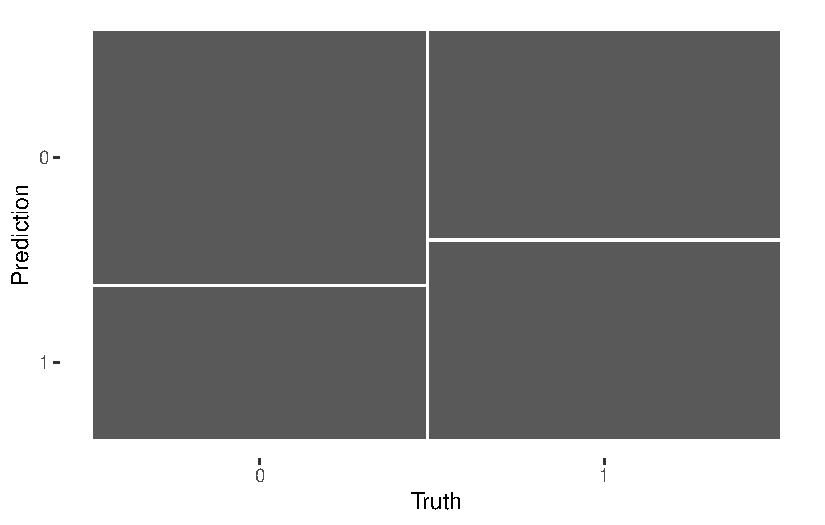
\includegraphics{assignment3_files/figure-pdf/LOGSTIC-Junyi-1.pdf}

}

\end{figure}



\end{document}
